% Interesting trick to instead make the chapter number the letter A for this appendix.
\begingroup
\renewcommand\thechapter{A}
\titleformat{\chapter}[display]
{\normalfont\huge\bfseries}{}{20pt}{\Huge}
\setcounter{section}{0} % Set the section counter back to 0 so the conclusion doesn't interfere.

\chapter*{Appendix A - EDA Process and Results}
\addcontentsline{toc}{chapter}{Appendix A - EDA Process and Results}
\markboth{Appendix A}{}
Problems identified through the EDA conducted in this Appendix were resolved in Section \ref{sec:Preprocessing}.

\section{Identification of missing or impossible values}
An initial glance at the dataset would make it appear as though as there are not any missing values in the dataset, as shown in Figure \ref{fig:InitialNoNAs}.

\begin{figure}[H]
    \centering
    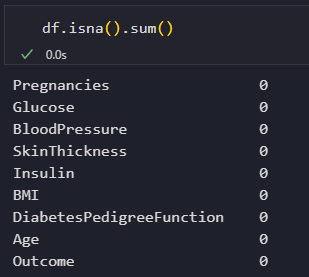
\includegraphics[width=.5\linewidth]{EDA/InitialNoNAs.png}
    \caption{An initial count of missing values before any further analysis.}
    \label{fig:InitialNoNAs}
\end{figure}

\para This would be very good - if it were true. Instead of missing values, this dataset contains impossible values in five columns, highlighted in red in 
Figure \ref{fig:ImpossibleValues}.\footnote{The mean of the outcome is highlighted in blue, as the fact that it is under 0.5 indicates that there are more 
cases of outcome 0 (no diabetes) than 1 (diabetes). This will be further analysed in Section \ref{sec:ImbalanceEDA}.}

\begin{figure}[H]
    \centering
    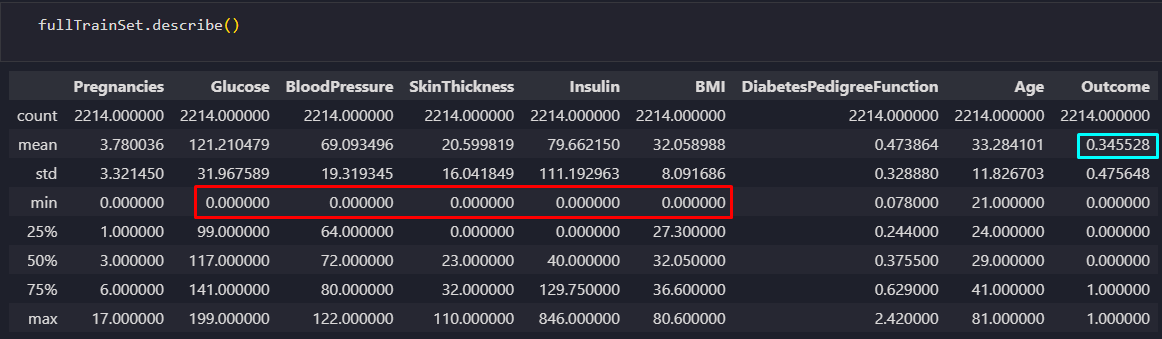
\includegraphics[width=\linewidth]{EDA/ImpossibleValues.png}
    \caption{The overall dataset description. Physically impossible values are \textcolor{red}{in red}.}
    \label{fig:ImpossibleValues}
\end{figure}

\para It is not possible for a living person to have a 0 in any of the five highlighted columns, and these datasets do not contain information of the deceased.
Therefore, it can be deduced that these values are erroneous, and should be treated as though they are missing. It is theorised by some in Kaggle discussions of these 
datasets that the zeroes in the Insulin column actually meant "imperceptible levels", which would have been useful data. However, a further review of literature around the datasets,
especially \textcite{hayashi_rule_2016}'s paper, led to the discovery that these zeroes truly are missing values that were missing due to experimental invalidity at the time 
of their collection.

\begin{figure}[H]
    \centering
    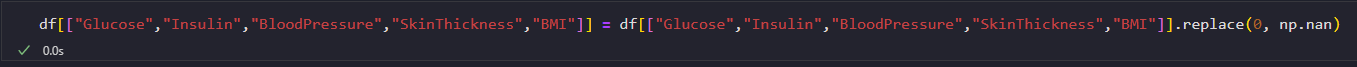
\includegraphics[width=\linewidth]{EDA/ConvertImpossibleValues-NoSums.png} % A version of this with NA sums exists too.
    \caption{Converting the impossible values to NaNs which are recognised by Pandas.}
    \label{fig:ConvertImpossibleValues}
\end{figure}

\para Now that there are officially recognised missing values, they can be visualised using the Missingno package, which can produce a 
matrix of missing values by column, seen in Figure \ref{fig:MissingnoMatrix}.
% bar chart of the amount of values in each column, seen in Figure \ref{fig:MissingnoBar}.

\begin{figure}[H]
    \centering
    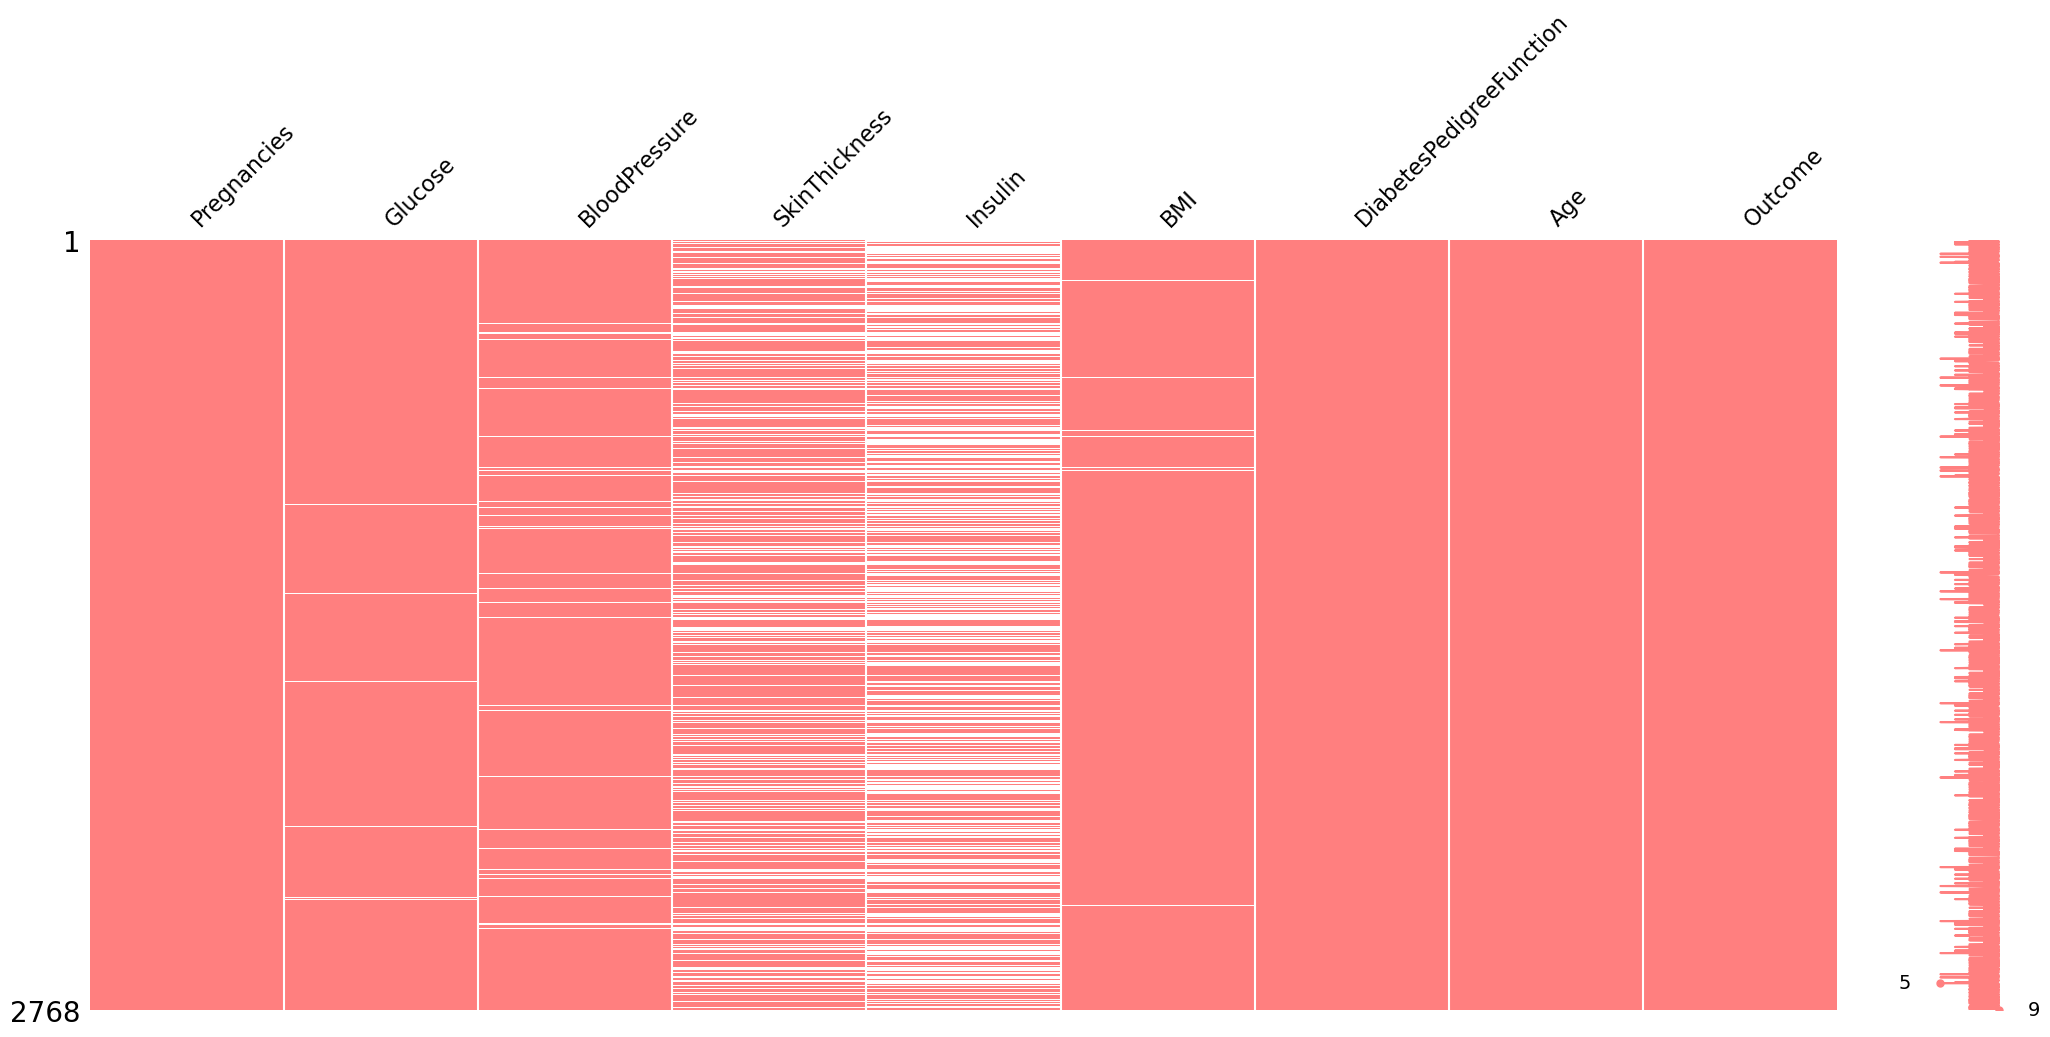
\includegraphics[width=\linewidth]{EDA/Plots/MissingnoMatrix.png}
    \caption{A Missingno matrix of the missing data per column.}
    \label{fig:MissingnoMatrix}
\end{figure}

% \begin{figure}[H]
%     \centering
%     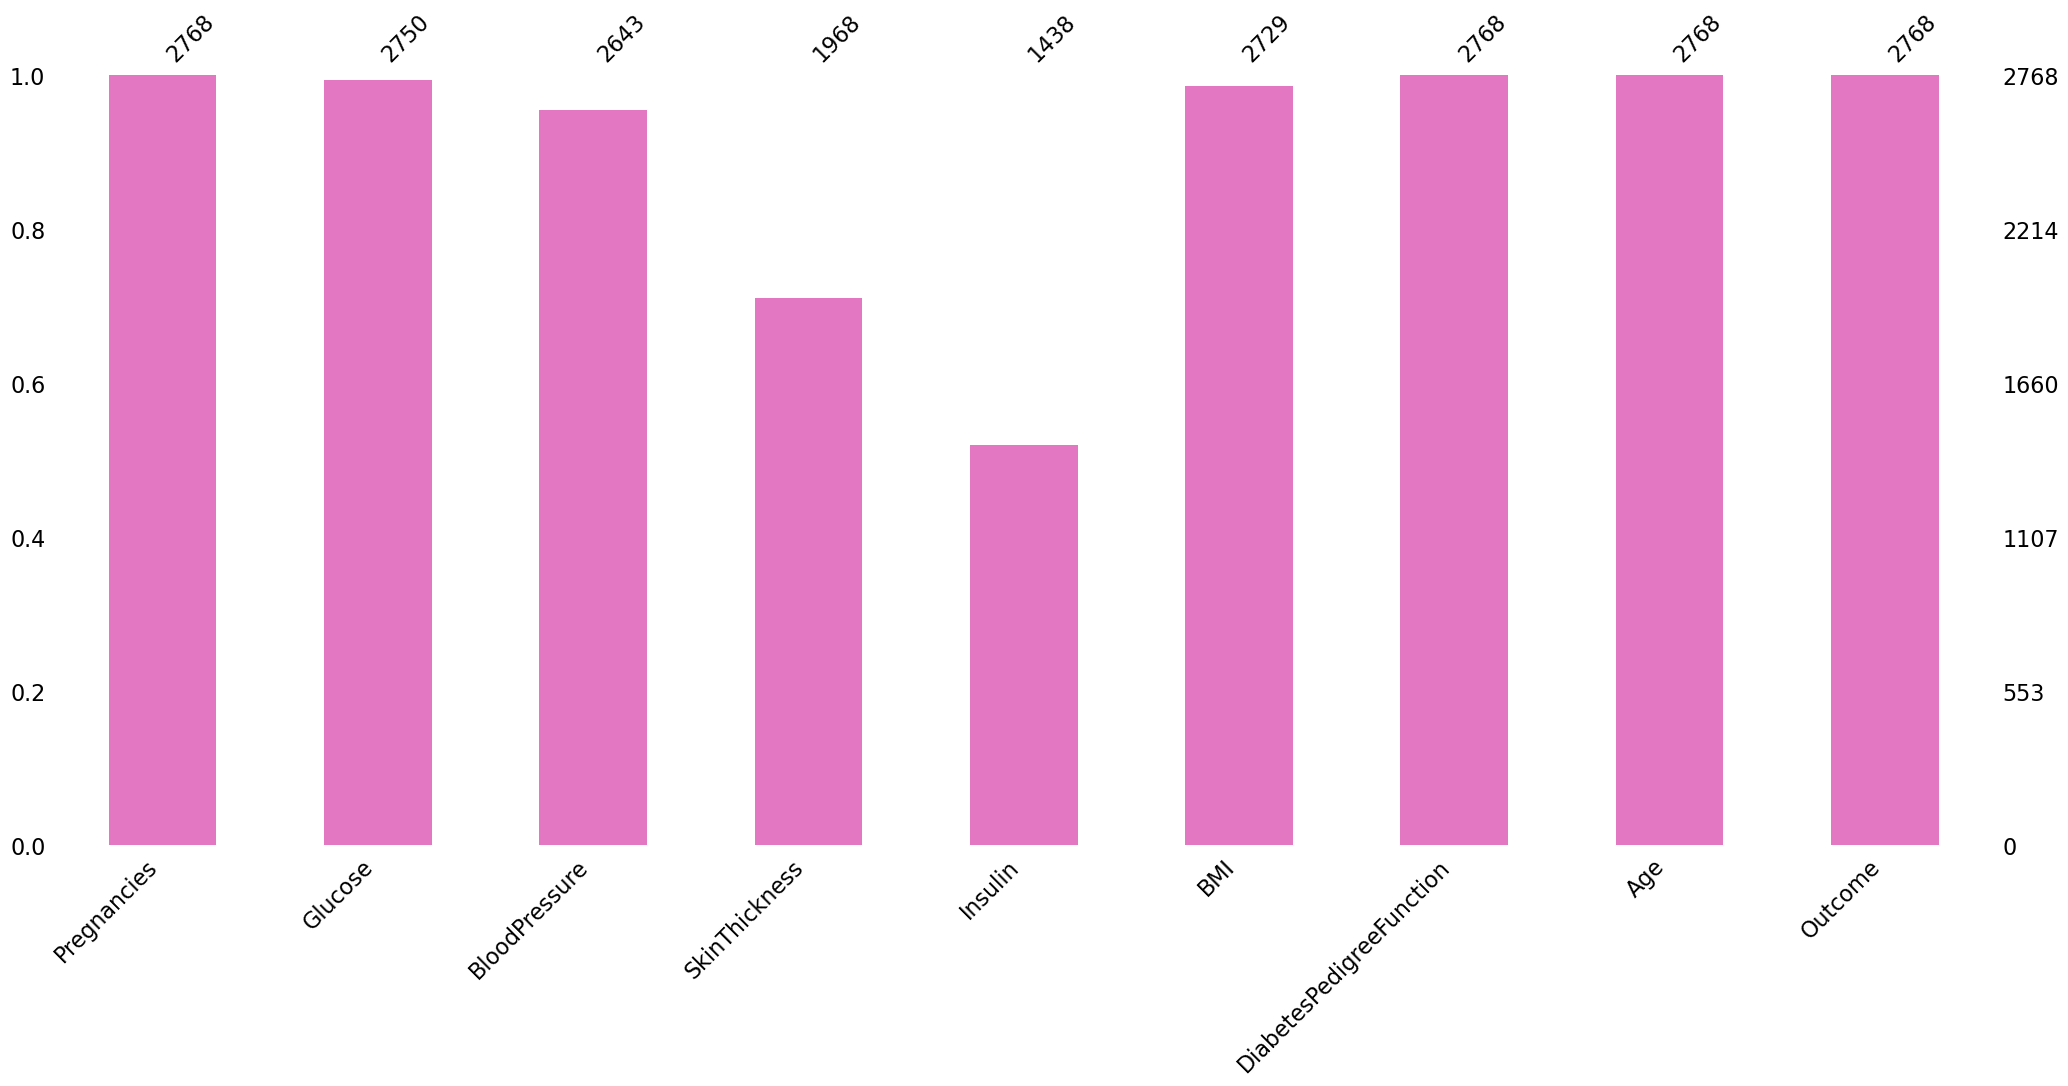
\includegraphics[width=\linewidth]{EDA/Plots/MissingnoBar.png}
%     \caption{A bar chart visualisation of the amount of data per column.}
%     \label{fig:MissingnoBar}
% \end{figure}

\para This matrix shows that the Insulin and SkinThickness columns contain considerable amounts of missing data alongside
many missing rows of BloodPressure, and some missing rows of BMI and Glucose, 
which will need to be fixed before any model can be trained. This is accomplished through imputation in Section 
\ref{sec:Preprocessing}.


\pagebreak 


\section{Target univariate analysis}
Binary classification models can develop bias if they do not have enough data of both classes to accurately predict what combinations 
of values should determine each class. Therefore, it is essential to view the balance between classes as in Figure \ref{fig:ClassImbalancePlot}.

\begin{figure}[H]
    \centering
    \includegraphics[width=.8\linewidth]{EDA/Code/TrainingValueCounts.png}
    \caption{The code to produce Figure \ref{fig:ClassImbalancePlot}.}
    \label{fig:ClassImbalancePlotCode}
\end{figure}

\begin{figure}[H]
    \centering
    \includegraphics[width=.6\linewidth]{EDA/Plots/TrainingValueCounts.png}
    \caption{The class distribution of the training set (0: 1449, 1: 765).}
    \label{fig:ClassImbalancePlot}
\end{figure}

\para The dataset is imbalanced, favouring an outcome of 0. The exact percentages 
of each class can be calculated as seen below.

\begin{equation}
    \text{Outcome 0} = \frac{1449}{2214} = 0.655 \times 100\% = 65.5\%
\end{equation}

\begin{equation}
    \text{Outcome 1} = \frac{765}{2214} = 0.345 \times 100\% = 34.5\%
\end{equation}

\para The training set is 80\% of the data, hence why it is 2214 rows rather than 2768. From these calculations, it can be determined that 
there is an imbalance present in the training set, and we can also assume there will be a similar imbalance in the unseen testing set, as the train\_test\_split method 
aims to maintain the original class balances where possible. The class imbalance will be resolved in Section \ref{sec:Preprocessing}.



\section{Multivariate analysis}
To compare each variable to each other and the outcome, a deep copy of the training 
set was created which merged X\_train and y\_train without affecting the originals.

\begin{figure}[H]
    \centering
    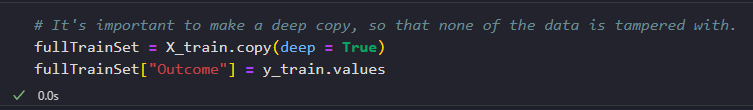
\includegraphics[width=.8\linewidth]{EDA/FullTrainingSet.png}
    \caption{Creating a variable to hold a copy of X\_train and y\_train.}
    \label{fig:FullTrainingSet}
\end{figure}

\subsection{Data distributions by Outcome}

It is important to identify significant outliers in the dataset so that models do not become skewed by the inflated variance, standard 
deviation and mean that they cause. Outliers that are very high in comparison to the primary distribution of the data will cause the 
standard deviation and mean to increase, whereas low outliers will make them decrease. Their identification is important not only for data analysis, 
but also for model development, as outliers can cause some algorithms to perform poorly or overfit, most notably distance-based algorithms 
such as K-Nearest Neighbours (KNN) and Support Vector Machines (SVM), which is further discussed in Section \ref{sec:ChosenAlgorithms}. 
% Source? It's true but cite something for that.

\para The simplest way to visualise outliers in the dataset is through box plots, which present the spread and skewness of numerical 
data in a simple visual format by showing the inter-quartile range (IQR), with rows outside of these being outliers. 
The boxplots of each column in the training set are shown below in Figure \ref{fig:AllBoxplotsByOutcome}. Each of the plots 
contains two boxplots, where one is for individuals without diabetes, and one is for those with diabetes.

\para In the figure, it can be seen that all columns contain some outliers.
However, most of these outliers are still relevant statistical data that would be possible, such as the outliers 
in Age being elderly people. Some of these outliers are less feasible, however; most notably the extreme high outliers 
in SkinThickness, BMI, and Insulin. Leaving these outliers in would affect the scaling of the data, and because it is generally 
ill-advised to remove rows of data especially with smaller datasets, they could instead be transformed to the upper bound to give 
a more even distribution. This will be accomplished in Section \ref{sec:Preprocessing}.

\begin{figure}[H]
    \centering
    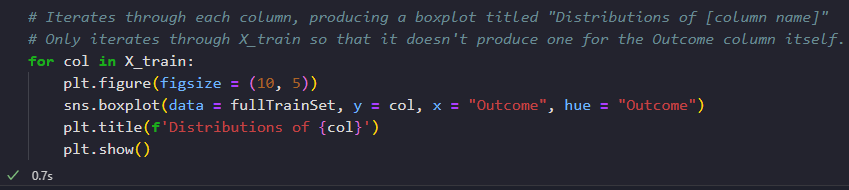
\includegraphics[width=\linewidth]{EDA/Code/BoxplotsByOutcome.png}
    \caption{The code used to produce Figure \ref{fig:AllBoxplotsByOutcome}.}
    \label{fig:BoxplotsByOutcomeCode}
\end{figure}


\begin{figure}[H]
    \centering
    % First row: 2 subfigures
    \begin{subfigure}[b]{0.45\textwidth}
        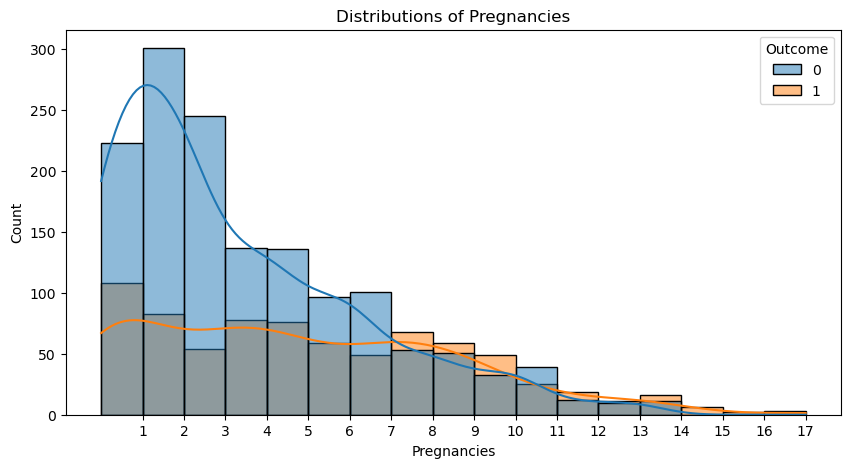
\includegraphics[width=\linewidth]{EDA/Plots/BoxplotsByOutcome/Pregnancies.png}
        \caption{Pregnancies}
        \label{fig:PregnanciesByOutcome}
    \end{subfigure}
    \hfill
    \begin{subfigure}[b]{0.45\textwidth}
        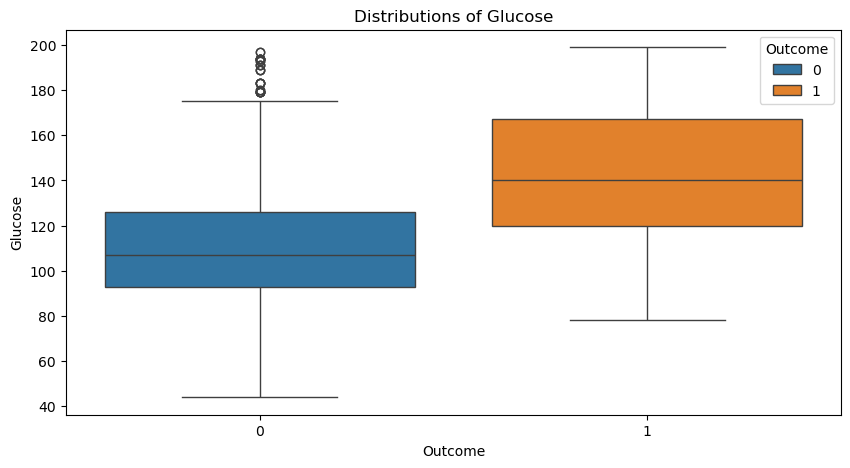
\includegraphics[width=\linewidth]{EDA/Plots/BoxplotsByOutcome/Glucose.png}
        \caption{Glucose}
        \label{fig:GlucoseByOutcome}
    \end{subfigure}
    
    \vspace{1em}
    
    % Second row: 2 subfigures
    \begin{subfigure}[b]{0.45\textwidth}
        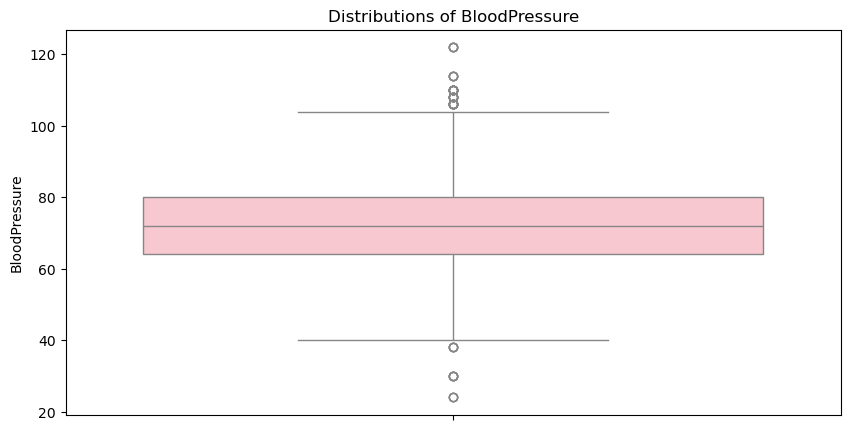
\includegraphics[width=\linewidth]{EDA/Plots/BoxplotsByOutcome/BloodPressure.png}
        \caption{BloodPressure}
        \label{fig:BloodPressureByOutcome}
    \end{subfigure}
    \hfill
    \begin{subfigure}[b]{0.45\textwidth}
        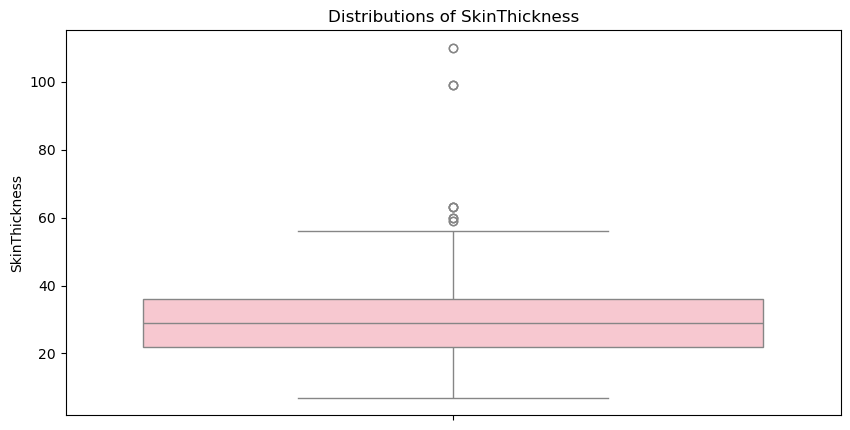
\includegraphics[width=\linewidth]{EDA/Plots/BoxplotsByOutcome/SkinThickness.png}
        \caption{SkinThickness}
        \label{fig:SkinThicknessByOutcome}
    \end{subfigure}
    
    \vspace{1em}
    
    % Third row: 2 subfigures
    \begin{subfigure}[b]{0.45\textwidth}
        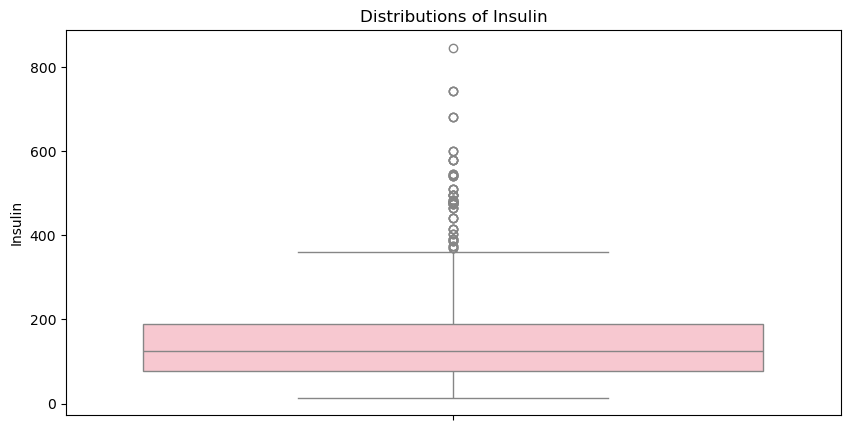
\includegraphics[width=\linewidth]{EDA/Plots/BoxplotsByOutcome/Insulin.png}
        \caption{Insulin}
        \label{fig:InsulinByOutcome}
    \end{subfigure}
    \hfill
    \begin{subfigure}[b]{0.45\textwidth}
        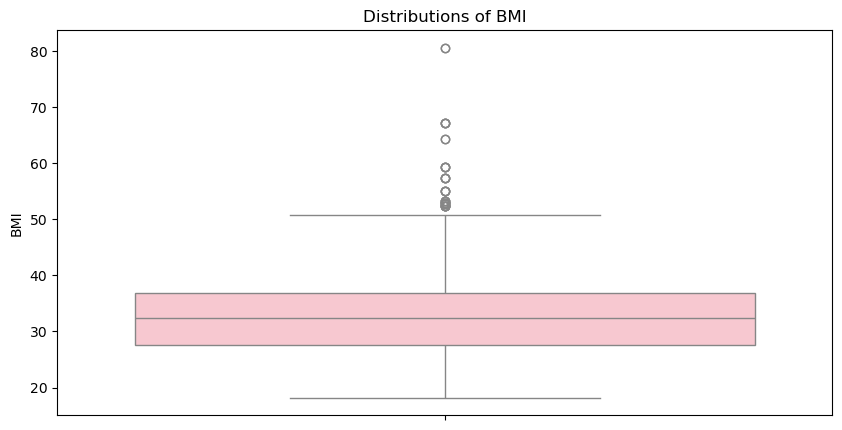
\includegraphics[width=\linewidth]{EDA/Plots/BoxplotsByOutcome/BMI.png}
        \caption{BMI}
        \label{fig:BMIByOutcome}
    \end{subfigure}
    
    \vspace{1em}
    
    % Fourth row: 2 subfigures
    \begin{subfigure}[b]{0.45\textwidth}
        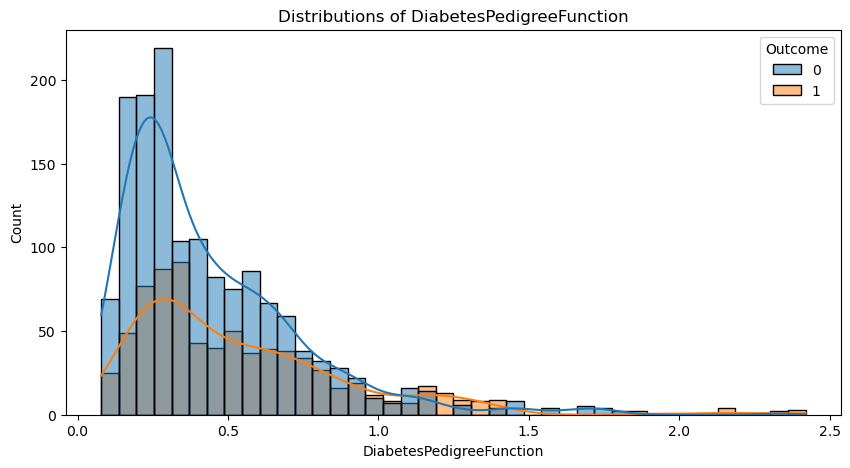
\includegraphics[width=\linewidth]{EDA/Plots/BoxplotsByOutcome/DiabetesPedigreeFunction.png}
        \caption{DiabetesPedigreeFunction}
        \label{fig:PedigreeByOutcome}
    \end{subfigure}
    \hfill
    \begin{subfigure}[b]{0.45\textwidth}
        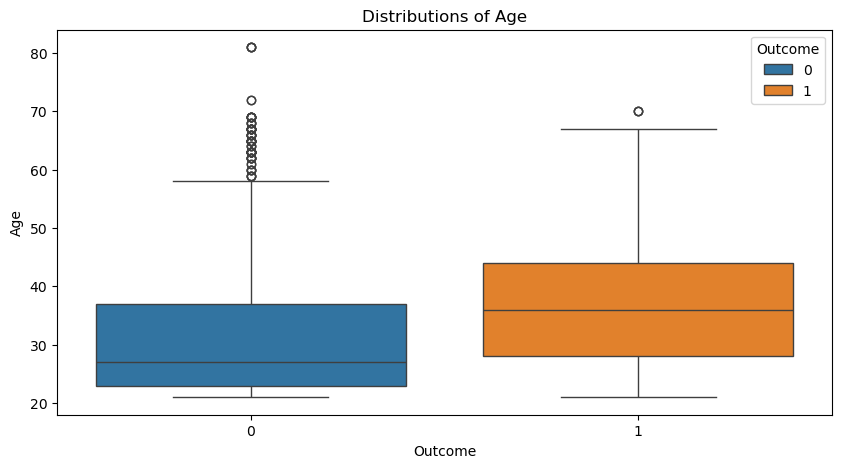
\includegraphics[width=\linewidth]{EDA/Plots/BoxplotsByOutcome/Age.png}
        \caption{Age}
        \label{fig:AgeByOutcome}
    \end{subfigure}
    
    \caption{Boxplots of all features by the outcome (Blue: No diabetes, Orange: Diabetes).}
    \label{fig:AllBoxplotsByOutcome}
\end{figure}

\pagebreak

\subsubsection{Pregnancies}
It was assumed in Table \ref{tab:Assumptions} that the amount of pregnancies a woman has had may bear a strong correlation
on whether they develop type 2 diabetes. This box plot does support the original assumption that the amount of pregnancies can positively 
correlate with the diabetes outcome, as the median and upper quartiles of the distributions of those with 
diabetes are higher than those without, though it also confirms that pregnancies are not a decisive factor 
on their own, as some patients had many pregnancies without having diabetes.

\subsubsection{Glucose}
This feature clearly shows a direct and strong correlation with the outcome; individuals with diabetes have
much higher glucose values, with a clear upward shift in both the median and interquartile range (IQR).
The lower whisker of the boxplots begins much higher with patients with diabetes, which implies that low glucose is a storng 
indicator that a patient does not have diabetes.

\subsubsection{BloodPressure}
Blood pressure values are fairly similar between the two groups, though individuals with diabetes show a slightly higher median.
Both groups have similar variability and range, indicating that blood pressure is not as strong a distinguishing factor. 
However, this slight correlation is still useful information, so this column should be kept. 

\subsubsection{SkinThickness}
This column contains significant outliers that will cause issues with data scaling.
Aside from these outliers, it does appear that skin thickness positively correlates with the outcome.

\subsubsection{Insulin}
This column contains many outliers, with some of these being extremely high. Aside from these, 
the main IQRs of the plots appear to indicate that higher insulin values are indicative of diabetes,
showing a positive correlation.

\subsubsection{BMI}
Individuals with diabetes tend to have higher BMI values on average.
The median BMI for the diabetic group is higher, with a slightly larger IQR, showing that BMI is an important factor in distinguishing diabetes outcomes.

\subsubsection{DiabetesPedigreeFunction}
The diabetes pedigree function has a slightly higher median for individuals with diabetes, but the difference is not substantial.
Both groups share significant overlap, suggesting that this feature alone may not strongly differentiate between outcomes, which 
differs from the original assumption.

\subsubsection{Age}
Individuals with diabetes tend to be older on average, as indicated by a higher median age for the diabetic group, and the fact that 
the IQR for the diabetic group is shifted upwards. However, many outliers without diabetes exist.

\subsection{Pair plot}
% This section is weak, though I don't know how best to improve it.
To view every column in the dataset plotted against each other, a pair plot can be created using Seaborn,
pictured in Figure \ref{fig:PairPlot}.

\begin{figure}[H]
    \centering
    \includegraphics[width=\linewidth]{EDA/Code/PairPlot.png}
    \caption{The code to produce Figure \ref{fig:PairPlot}.}
    \label{fig:PairPlotCode}
\end{figure}

\begin{figure}[H]
    \centering
    \includegraphics[width=\linewidth]{EDA/Plots/PairPlot.png}
    \caption{The pair plot of the full training set (Blue: No diabetes, Orange: Diabetes).}
    \label{fig:PairPlot}
\end{figure}

\para There are multiple observations on the relationships between features to be made from this pair plot, such as:
\begin{itemize}
    \item Glucose, BMI and Outcome 
        \begin{itemize}
            \item Glucose and BMI appear to be the two strongest predictors, with there being more cases of diabetes as each of these features increase,
            shown by the higher clustering of points. 
            \item Glucose also appears to slightly increase as BMI increases, suggesting a slight positive correlation between the two features. 
        \end{itemize}
    \item Pregnancies and Age
        \begin{itemize}
            \item As expected, pregnancies do typically increase with age. 
        \end{itemize}
    \item Pregnancies and Outcome
        \begin{itemize}
            \item There is no clear separation in the outcome based on pregnancies alone, suggesting it may not be a decisive factor.
        \end{itemize}
    \item Age
        \begin{itemize}
            \item While a person's age appears to not be directly relevant to them having diabetes, it instead appears that older individuals 
            instead typically have higher glucose levels and BMI, which are decisive factors.
        \end{itemize}
    \item Insulin
        \begin{itemize}
            \item Appears to be a good predictor, but not quite as much as glucose. Most rows where Insulin is between 400 and 600 are diabetic.
        \end{itemize}
    \item SkinThickness and BMI
        \begin{itemize}
            \item As expected, these two features are closely interlinked as seen by the mostly tight clustering between them in their associated plot.
        \end{itemize}
\end{itemize}

\subsubsection{Relation between Insulin and Glucose by Outcome}
A particular relation of note given the subject matter is the relation between insulin and glucose dependent on whether the 
individual has diabetes or not. Type 2 diabetes is characterised by insulin resistance and underproduction, meaning that lower insulin values are 
expected as glucose rises. Figure \ref{fig:ScatterInsulinGlucose} details this relation in patients with and without diabetes.

\begin{figure}[H]
    \centering
    \includegraphics[width=\linewidth]{EDA/Code/ScatterInsulinGlucose.png}
    \caption{The code to produce Figure \ref{fig:ScatterInsulinGlucose}.}
    \label{fig:ScatterInsulinGlucoseCode}
\end{figure}

\begin{figure}[H]
    \centering
    \includegraphics[width=\linewidth]{EDA/Plots/ScatterInsulinGlucose.png}
    \caption{A scatter plot with lines of best fit to show the trends in Insulin and Glucose.}
    \label{fig:ScatterInsulinGlucose}
\end{figure}

\para The expectation is matched, as glucose rises more than insulin in patients with diabetes, and slower 
than insulin in patients without diabetes.



\subsection{Correlation Matrix}
An alternative and simpler way to visualise the correlations between features in a dataset is through a correlation matrix as 
pictured in Figure \ref{fig:CorrMatrix}. The matrix uses the full training set created earlier to show the correlations between 
the dataset's features in an annotated heatmap format, quantifying each correlation as a number. Correlation matrices only work with numerical features, 
though all features are numeric in this dataset which enables the matrix to show all features. 

\begin{figure}[H]
    \centering
    \includegraphics[width=\linewidth]{EDA/Code/CorrelationMatrix.png}
    \caption{The code to produce Figure \ref{fig:CorrMatrix}.}
    \label{fig:CorrMatrixCode}
\end{figure}

\begin{figure}[H]
    \centering
    \includegraphics[width=\linewidth]{EDA/Plots/CorrelationMatrix.png}
    \caption{The correlation matrix of the full training set.}
    \label{fig:CorrMatrix}
\end{figure}

\para The correlation matrix reflects many of the observations noted in the pair plot and data distributions.
It shows the relationships between all features, including many expected relations like those of Glucose and Outcome,
Pregnancies and Age, and BMI and SkinThickness. However, the matrix also reveals insights that subvert the previous 
assumptions about the dataset, such as the pedigree function actually having the weakest correlation with the outcome.
This can be explained through other insights in the data as well as academic research.

\para \textcite{mambiya_play_2019} argue that diabetes mellitus can be caused by genetic predisposition, which is 
represented by the pedigree function in this dataset, though lifestyle factors such as weight gain and poor dietary 
variance can be a more significant factor in the cause of the disease in both those with and without genetic predispositions.
Their findings are also echoed within this dataset, with high BMIs representing overweightiness/obesity and high Glucose values representing 
high sugar intake, which are the two most significant factors in the outcome according to the correlation matrix.

\endgroup